\chapter{Desenvolvimento}
	\chapterprecis{Este capítulo apresenta o desenvolvimento do sistema objetivo deste trabalho. São apresentadas as decisões de projeto, arquitetura e alguns trechos não triviais do códigos são explicados}
	
	\section{Decisões de Projeto}
		O estado atual do trocador de calor foi descrito na \autoref{sec:trocador}. O intuito deste projeto é implementar um sistema de monitoramento e controle remoto sem que haja alteração da infraestrutura já instalada. Em resumo, o objetivo é incluir algum dispositivo que necessite apenas se comunicar com o Arduino para executar suas tarefas.
		
		Para este projeto, é possível utilizar tanto uma arquitetura SCADA tradicional, quanto tecnologias embarcadas como placas de prototipagem. Foi definido utilizar a segunda opção, devido a fatores econômicos e também pela portabilidade concedida ao sistema. A arquitetura foi inspirada em grande parte no sistema BrewPi, descrito na \autoref{sec:exemplos}. O Raspberry Pi 3 foi escolhido por possuir comunicação Wifi integrada à placa, e possuir uma documentação mais extensa que outras placas similares no mercado como o BeagleBone Black\footnote{\url{https://beagleboard.org/black}} e a recente e também poderosa placa DragonBoard 410c\footnote{\url{https://developer.qualcomm.com/hardware/dragonboard-410c}}. Dessa forma, a visão geral do sistema proposto é exibida na \autoref{fig:arq_proposta}.
		
		\begin{figure}[!htb]	
			%\centering
			\captionsetup{justification=centering}
			\begin{center}
				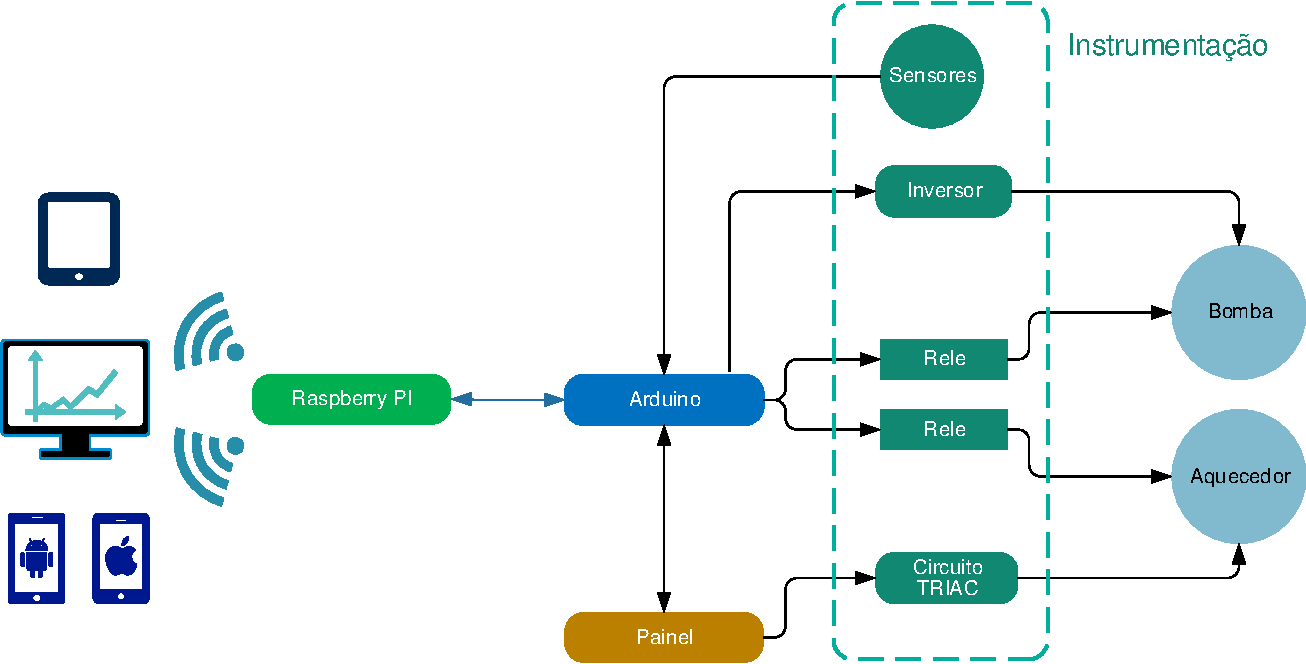
\includegraphics[width=14cm]{arq_proposta}  %pode alterar o tamanho
				\caption[Nova Arquitetura Proposta para o Sistema]{\label{fig:arq_proposta} Nova Arquitetura Proposta para o Sistema }
			\end{center}	
		\end{figure}
	
	\section{Requisitos Funcionais do Sistema}
		Uma vez definido o hardware a ser utilizado, deve-se levantar os requisitos funcionais do sistema, ou seja o que o sistema deve fazer e como deve reagir em determinadas situações. Basicamente, os requisitos funcionais são as características de operação do sistema de monitoramento a ser desenvolvido. Os requisitos estão resumidos na \autoref{tbl:requisitos}.
			
		\begin{table}[!htb]
			\centering
			\caption{Requisitos Funcionais do Sistema}
			\label{tbl:requisitos}
			\def\arraystretch{1.3}
			\begin{tabular}{c p{11cm}}
				\hline
				\multicolumn{1}{c}{\textbf{Índice Requisito}} & \multicolumn{1}{c}{\textbf{Descrição Requisito}} \\ \hline 
				1 & Exibir a informação atual das variáveis de processo (vazões e temperaturas) \\ %\hline
				2 & Exibir o estado da bomba e do aquecedor (Ligado ou Desligado) \\ %\hline  
				3 & Exibir o valor da rotação atual da bomba \\ %\hline
				4 & Em modo remoto, deve permitir que o operador acione a bomba e o aquecedor \\ %\hline
				5 & Em modo remoto, deve permitir que o operador altere a velocidade da bomba \\ %\hline
				6 & Permitir a visualização dos dados analógicos em gráficos \\ %\hline
				7 & Impedir a atuação do operador quando o Arduino estiver em modo local ou de emergência \\ %\hline
				8 & Armazenar os dados do sistema em banco de dados \\ %\hline
				9 & Permitir que o usuário habilite ou desabilite o armazenamento de dados das variáveis \\ %\hline
				10 & Permitir que o usuário colete as informações contidas no banco em um arquivo no formato csv \\ %\hline
				11 & Permitir que o usuário apague as informações contidas no banco de dados \\ \hline
			\end{tabular}
		\end{table}
		
		\subsection{Descrição Funcional}
			Para atender aos requisitos citados acima, optou-se por modularizar as funcionalidades do sistema. Dessa forma, foram definidos 3 componentes. O termo componente deve ser entendido como um programa. Os componentes foram projetados de forma que cada um funcione de forma mais independente possível. Assim, o impacto no sistema caso haja alguma alteração de componente, em termos de reengenharia, é minimizado.
			
			A relação entre os componentes é exibida na  \autoref{fig:arq_componentes}. Foram definidos 3 componentes: o programa que é executado no Arduino; o Gateway e o WebServer, que são programas executados no Raspberry. Optou-se por criar dois componentes no Raspberry PI, de forma que as funcionalidades do sistema fossem corretamente agrupadas. As atribuições de cada programa estão resumidas na \autoref{tbl:atribuições}.
			
			\begin{figure}[!htb]	
				%\centering
				\captionsetup{justification=centering}
				\begin{center}
					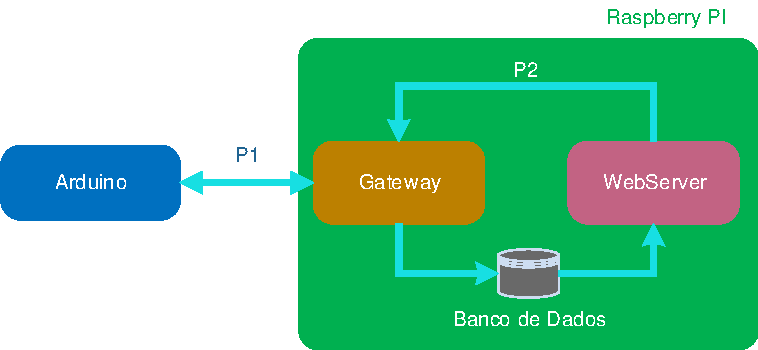
\includegraphics[scale=0.7]{arq_componentes}  %pode alterar o tamanho
					\caption[Arquitetura Detalhada]{\label{fig:arq_componentes} Arquitetura Detalhada }
				\end{center}		
			\end{figure}
			
			\begin{table}[!htb]
				\centering
				\captionsetup{justification=centering}
				\caption[Atribuições de cada Componente]{Atribuições de cada Componente}
				\label{tbl:atribuições}
				\def\arraystretch{1.3}
				\begin{tabular}{m{2cm}| p{12cm}}
					& \multicolumn{1}{c}{\textbf{Atribuições}} \\ \hline
					
					\multirow{4}{*}{Arduino} 
					& 1 - Interface com sensores e Atudadores \\
					& 2 - Interface com Painel \\
					& 3 - Enviar estado do sistema quando solicitado pelo Gateway\\
					& 4 - Interpretar comandos enviados pelo Gateway \\ \hline
					
					\multirow{3}{*}{Gateway} & 5 - Solicitar de forma cíclica o estado das variáveis \\
					& 6 - Armazenar os dados recebidos em um banco de dados \\
					& 7 - Receber comandos vêm do WebServer (comandos dos usuários) e repassar ao Arduino \\ \hline
					
					\multirow{2}{*}{WebServer} & 8 - Ler dados do banco e apresentar ao usuário \\
					& 9 - Receber comandos do usuário e repassar ao Gateway \\
					
					\hline
				\end{tabular}
			\end{table}
		
			É importante observar que o Gateway apenas cuida da transferência de informações entre WebServer e Gateway. O programa contém duas threads: uma para realizar a solicitação cíclica de dados ao Arduino e armazená-los no banco de dados; e a outra para aguardar o envio de comandos vindos do WebServer e repassar ao Arduino.  A comunicação entre Gateway e Arduino é realizada através do protocolo I2C, e a comunicação entre Gateway e WebServer é feita através de sockets TCP/IP.
			
			O sistema foi projetado de forma que a substituição de um componente não influencie os demais, contudo alterações nos protocolos influenciaria o código dos componentes envolvidos. Portanto os protocolos devem ser mantidos.
			 
	\section{Implementação}
		Essa seção consiste em detalhar o funcionamento dos componentes e a comunicação entre eles. Alguns trechos de códigos, considerados não triviais são explicados.
		
		\subsection{Arduino}
			\label{Arduino}
			O código fonte completo está disponibilizado no Github\footnote{\url{https://www.oficinadanet.com.br/post/14791-o-que-github}}, no link \url{https://github.com/felipefonsecabh/ArduinoCode/blob/ArduinoNoNavigation/ArduinoCode.ino}
			
			Foi feita uma análise do programa atual que o Arduino executa. O programa é extenso (contém 1482 linhas), sendo que cerca de 90\% do código é dedicado a cuidar do sistema de navegação do display LCD através dos botões existentes no painel.  A implementação de um sistema de monitoramento elimina a necessidade dessa estrutura de navegação, de modo que o painel passe a ter apenas funcionalidades diretas de acionamento, e o display exiba apenas informações básicas. Portanto, a melhor opção foi reformular o código do Arduino e aproveitar apenas as funções que fazem a leitura dos sensores e convertem os valores para unidade de engenharia. Essas funções se fazem necessária, pois não é escopo do projeto recalibrar sensores e/ou alterar a instrumentação já existente.
				
			A estrutura do código, que está exibida na \autoref{fig:fluxo_arduino}, foi montada de forma a permitir rápida adaptação do mesmo para diferentes protocolos de comunicação, e está de acordo com as atribuições mencionadas na \autoref{tbl:atribuições}. As trocas de mensagens com o Gateway são feitas por interrupção, ou seja, estão fora da função \textit{loop} do Arduino. 
				
			O programa foi intensamente modularizado. Todos os estados e funcionalidades foram encapsuladas em funções. Esse tipo de prática acelera a interpretação do código. Outro benefício é a possibilidade de expansão de funcionalidades, como por exemplo a implementação de malhas de controle no código. 
				
			No diagrama é utilizado o termo ``estado do sistema'', que deve ser interpretado como o conjunto de variáveis necessários para descrever o sistema. Essas variáveis são: as 4 temperaturas; 2 vazões; estado de acionamento de bomba e aquecedor (Ligado ou Desligado); velocidade da bomba; modo de operação (Local ou Remoto) e se o botão de emergência está acionado ou não.
			
			\begin{figure}[!htb]	
					%\centering
					\captionsetup{justification=centering}
					\begin{center}
						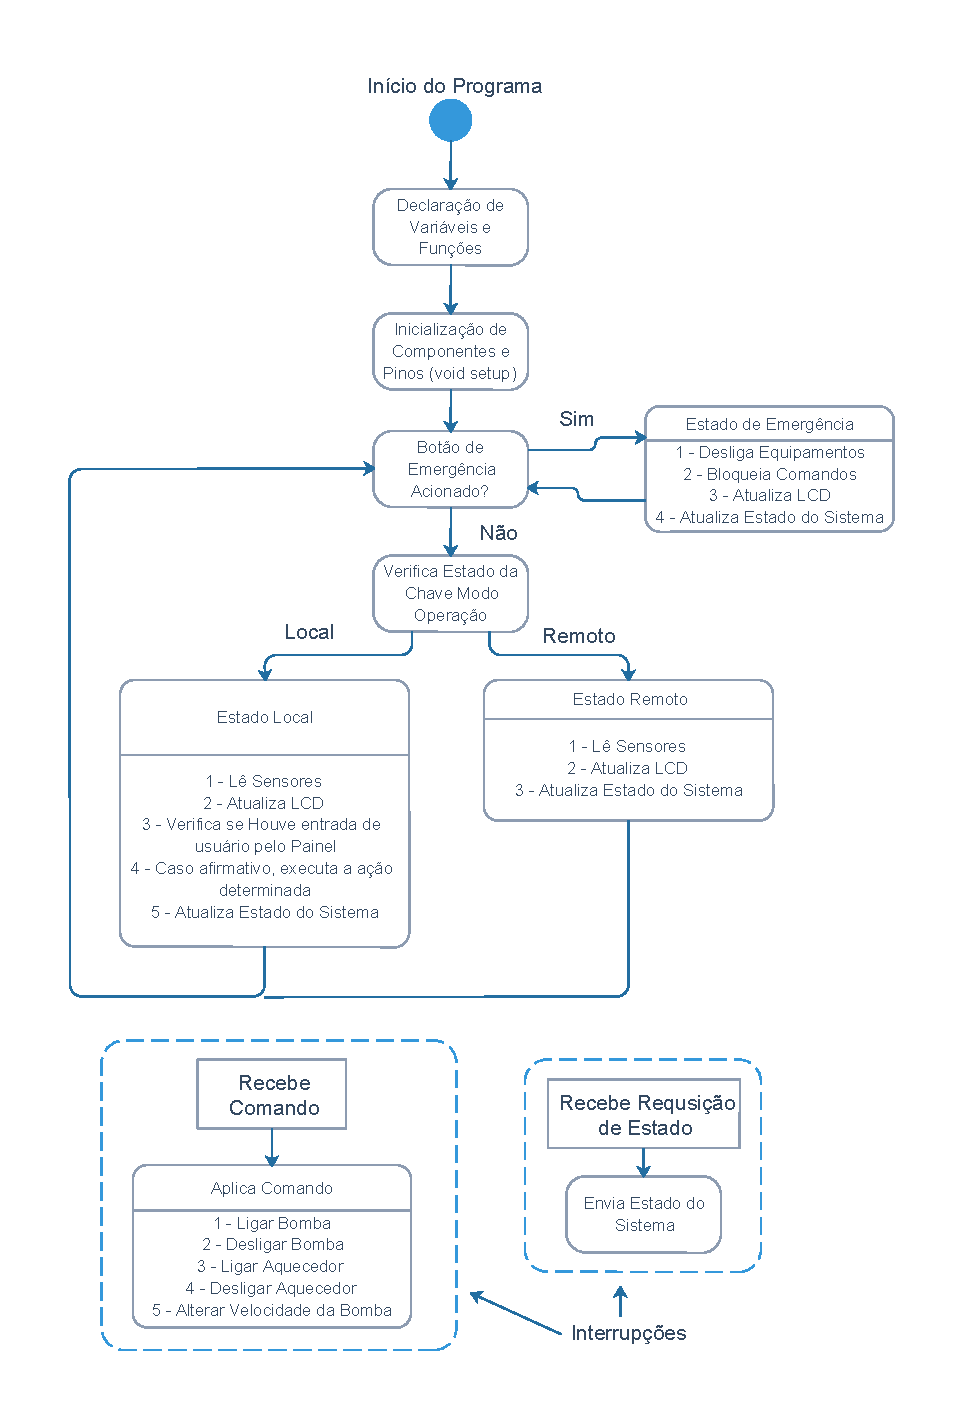
\includegraphics[width=12cm]{fluxo_arduino}  %pode alterar o tamanho
						\caption[Estrutura do Código do Arduino]{\label{fig:fluxo_arduino} Estrutura do Código do Arduino }
					\end{center}		
			\end{figure}
			
			Para a leitura dos sensores foram utilizadas bibliotecas desenvolvidas e mantidas por terceiros. A \autoref{tbl:libs} mostra a relação entre tabelas, desenvolvedores e versões. Não foi necessária nenhuma biblioteca para a leitura da vazão de água fria. O sensor de vazão consiste em um dispositivo que envia pulsos ao Arduino. Quanto mais pulsos enviados, maior é a vazão. Portanto, é feita uma contagem de pulsos em um intervalo de tempo fixo, e posteriormente esse número é inserido em uma fórmula que retorna o valor da vazão. A contagem de pulsos é feita por interrupção.
			
			O código correspondente a leitura dos valores analógicos é mostrado no \autoref{cod:read_arduino}.
			
			\begin{table}[!htb]
				\centering
				\captionsetup{justification=centering}
				\caption[Bibliotecas utilizadas no programa do Arduino]{Bibliotecas utilizadas no programa do Arduino}
				\label{tbl:libs}
				\def\arraystretch{1.3}
				\begin{tabular}{l c l l}
					\hline
					\textbf{Biblioteca} & \textbf{Versão}& \textbf{Mantida por} & \textbf{Função} \\ \hline
					Dallas Temperature & v3.7.6 & \textcite{miles2016} & Temperatura \\
					OneWire & v2.3.3 & \textcite{paul2017} & Temperatura \\
					Ultrasonic & - & \textcite{filipeflop2011} & Vazão Quente \\					
					\hline
				\end{tabular}
			\end{table}
		
			\begin{listing}[!htb]
				\begin{minted}[bgcolor=bg,breaklines=true,tabsize=2, baselinestretch=1,fontsize=\footnotesize]{cpp}
				void Temperaturas() {
					// call sensors.requestTemperatures() to issue a global temperature 
					// request to all devices on the bus
					sensors.requestTemperatures();
				
					// print the device information
					for (byte i = 0; i <= 4; i++){
						temp[i] = sensors.getTempC(deviceID[i]);
					}
				}
				
				void VazaoAguaFria(){
					currentTime = millis();
					// Every second, calculate litres/hour
					if (currentTime >= (cloopTime + 1000)){
						cloopTime = currentTime; // Updates cloopTime
						// Pulse frequency (Hz) = 7.5Q, Q is flow rate in L/min.
						vazao_fria = (flow_frequency / 7.5); // (Pulse frequency) / 7.5Q = flowrate in L/min
						flow_frequency = 0; // Reset Counter
					}
				}
				
				void VazaoAguaQuente(){
					float vazao1_sf; //descobrir o porque do nome da variavel
					microsec = ultrasonic.timing();
					cmMsec = ultrasonic.convert(microsec, Ultrasonic::CM);
					nivel = 11.46 - cmMsec;
					vazao1_sf = (0.0537)* pow((nivel * 10), 1.4727);
					if (vazao1_sf > 1){
						vazao_quente = 0.75*vazao_quente + 0.25*vazao1_sf;
					}
				}	
				\end{minted}
				\caption{Funções de Leitura dos sensores}
				\label{cod:arduino}
			\end{listing}
			
			A troca de dados entre Arduino e Gateway é feita pelo protocolo I2C. Este protocolo é implementado no Arduino através da biblioteca Wire. Neste projeto o Arduino atua como slave da comunicação, ou seja, não inicia a comunicação. Responde a algum dispositivo mestre apenas quando solicitado.
			 
			Quando o mestre envia um comando de escrita, atua-se uma interrupção, que executa a função onReceive. Quando o mestre envia uma solicitação de dados, atua-se uma outra interrupção, que executa a função onReceive e posteriormente executa a função onRequest. Em suma, a função onReceive é utilizada para interpretar comandos, como por exemplo ligar ou desligar bomba e aquecedor, e a função onRequest é utilizada para enviar para o mestre dados sobre o processo como por exemplo valores de temperaturas e vazões.
			
			As informações no protocolo I2C trafegam sob a forma de um array de bytes. Portanto, as informações referentes ao sistema, que são booleanas e reais, devem ser convertidas em um array de bytes para serem transmitidas.  É possível realizar essa conversão utilizando a declaração union. Essa técnica permite que variáveis de diferentes tipos ocupem uma mesma região de memória. Assim, foi criada uma estrutura de dados para representar o estado do sistema, que compartilha essa região de memória com um array de bytes. O \autoref{cod:dadosi2c} corresponde a essa implementação feita.
			
			\begin{listing}[!htb]
				\begin{minted}[bgcolor=bg,breaklines=true,tabsize=2, baselinestretch=1,fontsize=\footnotesize]{cpp}
				//estrutura de dados para envio i2c
				typedef struct processData{
					float temp1;
					float temp2;
					float temp3;
					float temp4;
					float hotflow;
					float coldflow;
					float pump_speed;
					byte bstatus;
					byte chksum;
				};
				
				typedef union I2C_Send{ //compartilha a mesma área de memória
					processData data;
					byte I2C_packet[sizeof(processData)];
				};				
				\end{minted}
				\caption{Estrutura de dados do sistema}
				\label{cod:dadosi2c}
			\end{listing}
			
			Em relação ao recebimento de comandos pelo Gateway, primeiramente é necessário entender como é a estrutura de um frame enviado pelo mestre. A estrutura do frame está descrita na \autoref{fig:i2c_packet}.
			
			\begin{figure}[!htb]	
				%\centering
				\captionsetup{justification=centering}
				\begin{center}
					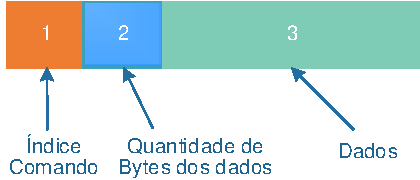
\includegraphics[scale=0.9]{i2c_packet}  %pode alterar o tamanho
					\caption[Estrutura de um pacote I2C]{\label{fig:i2c_packet}Estrutura de um pacote I2C}
				\end{center}		
			\end{figure}
		
			O ínidice de comando arbitrário e é definido pelo desenvolvedor. Portanto, para interpretar corretamente os comandos pelo mestre, foi necessário mapear ações de acrodo com o índice de comando criado, ou seja, definir um protocolo básico de comunicação. A relação entre o índice de comando e a ação correspondente é mostrada na \autoref{tbl:comandos}.A interpretação e execução dos comandos é feita na função onReceive. Se o comando é uma solicitação de dados, o envio é realizado na função onRequest.
			
			\begin{table}[!htb]
				\centering
				\caption{Definição das interpretações de comando}
				\label{tbl:comandos}
				\def\arraystretch{1.3}
				\begin{tabular}{c c l}
					\hline
					\textbf{Comando (Char)} & \textbf{Comando (Decimal)} & \textbf{Ação}  \\ \hline
					
					`1' & 49 & Ligar a bomba \\ %\hline
					`2' & 50 & Desligar a bomba \\ %\hline  
					`3' & 51 & Ligar aquecedor \\ %\hline
					`4' & 52 & Desligar o aquecedor \\ %\hline
					`5' & 53 & Alterar velocidade da bomba \\
					`6' & 54 & Enviar dados do sistema para o mestre \\ %\hline
					\hline
				\end{tabular}
			\end{table}
		
		Foi colocada a representação decimal e em char dos comandos, porque no Arduino o comando é interpretado na forma decimal, enquanto no Gateway os comandos são interpretados como char. A relação entre o valor em char e decimal é dada pela tabela ASCII\footnote{\url{https://en.wikipedia.org/wiki/ASCII}}.
		
	\subsection{Preparação do Raspberry}
			